%PUT STG, COG, ADG as option
\documentclass[COG,11pt]{ercgrant}
% put here the year of the call
\renewcommand{\callyear}{2023}
\setmainfont{Arial}
\bibliography{bibliography.bib}
% \bibliography{nature-refs.bib}

\author{Fabian Sinz}
\acro{Visual System in Action}
% \title{Putting data-driven digital twins of mouse visual cortex into action.}
% \title{Towards a meta-verse for the mouse visual system}
\title{Building a data driven model how behavior changes neuronal processing in mouse visual cortex in freely behaving mice}
\institution{Georg August Universität Göttingen Stiftung Öffentlichen Rechts}

% ====== BODY OF THE DOCUMENT ======
\begin{document}

\maketitle

\begin{abstract}
	\textcolor{red}{
		Sensory systems are our window to the world and form the basis for our decisions and behavior. 
However, sensory processing is not a one-way street:
Motor behavior and the internal state of an animal can alter how sensory signals are processed.
Even in head-restrained animals, previous studies found a rich influence of motor behavior on neural activity. 
How and when the brain adjusts sensory processing during unconfined real-world  behavior in complex natural environments is currently unknown. 
I hypothesize that, under these conditions, the brain dynamically adjusts sensory processing to the current behavioral context not only by changing the gain, but the selectivity of sensory neurons. 
I further hypothesize that these changes momentarily increase the reliability of relevant environmental aspects in neuronal representations. 

I will investigate this in the visual system of mice by building deep data-driven functional twin models of visual cortex and behavior in digital replicas of real experimental environments.
The models will be trained on a massive dataset of recordings from excitatory neurons from nine areas of visual cortex in head-fixed and freely behaving mice under spontaneous and task-driven behavior.
I will use these twins to discover which neurons change their tuning, how and under which behavioral context they change it, and how the animal's behavior would be different if these mechanisms were shut down.
If successful, this project will not only change our view on how the visual system adapts to behavior under natural conditions, but also yield a computational framework with a vast range of applications in neuroscience. 
It is straightforward to generalize to other areas, stimulus modalities, and species, and will be an enabling tool to study how the brain makes sense of the environment in unconfined behaving animals.

% in real world tasks
 % -- not only changing the gain, but also the selectivity of single sensory neurons
	}
\end{abstract}


%%%%%%%%%%%%% EXTENDED SYNOPSIS %%%%%%%%%%%%%%%%%%%

\section{Extended Synopsis of the Scientific Proposal}

\subsection{Background, state of the art and rationale}
% Visual features are often only hypothesized to play a role. Behavioral verification is missing
The goal of the visual system is to extract actionable information about our environment from the complex and ambiguous light patterns that inform our brain about the world beyond our eyes.
However, vision is not a one-way street: The activity of each neuron in the visual system is not only determined by visual input, but also changes with the internal or behavioral state of the animal~\parencite{Niell2010-bs, Musall2019-kd, Erisken2014-un, Franke2022-do}. 
However, almost all previous work on the influence of behavior on the representation\footnote{In the following I will use the terms \textit{tuning}, \textit{(en)coding}, and \textit{representation} to denote how neurons respond to visual stimuli, \textit{i.e.} their response function \texttt{activity = f(visual input)}.} of visual stimuli have been performed with restrained animals, attached to the experimental recording device.
Consequently, a characterization of how visual representations are modulated under freely viewing and behaving animals is missing. 
The goal of this proposal is to \textbf{investigate the hypothesis that neurons in mouse visual cortex change their tuning function to visual stimuli with the behavioral context to decrease the uncertainty about relevant aspects of the world. To this end, I will build a computational framework based on data-driven deep neural network models of the visual system, detailed motor behavior captured by skeleton graphs of freely behaving mice, digitized real environments and reinforcement learning.} 

% To understand behaviorally relevant visual processing, we need to move towards a \textbf{natural neuroscience} that studies a system in an environment it was made for~\parencite{Huk2018-ez, Datta2019-qj}.
To study how behavior influences visual processing, we need to characterize how the response of neurons in the visual systems changes in freely behaving (unrestrained) animals using visual stimuli that engage the computational apparatus of the visual system~\parencite{Huk2018-ez, Datta2019-qj}. 
While the vast majority of visual neuroscience still uses head-fixed animals there is a trend towards large scale recordings in freely behaving animals~\parencite{Parker2022-ac}.
% , even though the number of simultaneously observable neurons in freely behaving animals is still one to two orders of magnitude lower.
However, using them to study the effect of behavior on neuronal tuning poses new challenges:
% However, this data poses new challenges:
\circled[midblue][midblue][white]{1} We need to disentangle the contributions of the stimulus, the behavior, and the internal state of the animal to the activity of neurons during free behavior. 
This includes reconstructing what the animal saw at every moment of the experiment, and developing models that can capture common fluctuations in neuronal population activity.
\circled[midblue][midblue][white]{2} To characterize how neuronal tuning changes with behavior in a classical experimental trial structure, one would need to present the same stimuli in different behavioral contexts. 
However, behavior and visual input in natural conditions cannot easily be controlled or repeated, and the stimulus is not easily parametrized.
This creates the need for a computational framework to compile behavioral and physiological observations (possibly from multiple experiments) into a single computational model -- a \textbf{functional twin}\footnote{I will use the term \textit{functional twin} for a model that can faithfully predict measurable observations for a real system, such as neural activity or behavior, over a large range of conditions, \textit{e.g.} arbitrary videos or behaviors. A functional twin mimics the system \textit{functionally}, without necessarily resembling it \textit{structurally}. } -- that allows us to characterize tuning \textit{in silico} and make specific predictions that are testable \textit{in vivo}.

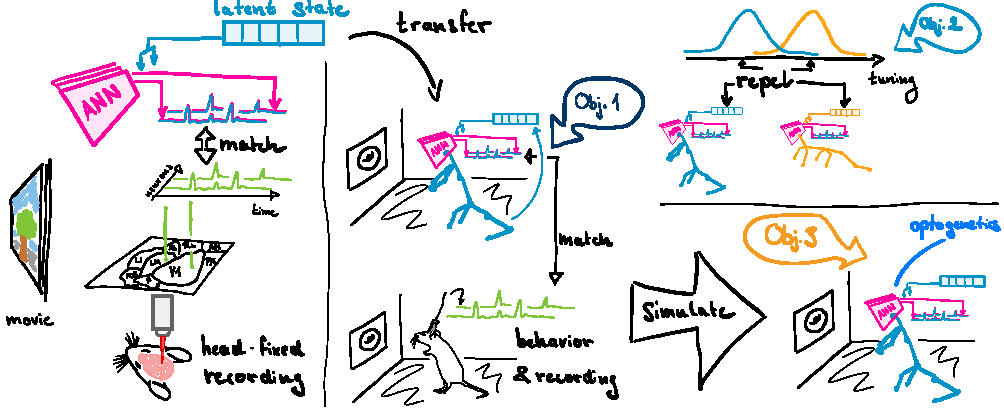
\includegraphics[width=\textwidth, height=7cm]{figures/overview.pdf}

That sensory responses are modulated by the animal's motor activity and internal state, such as attention, is documented for many species \parencite{Rowell1971-zj, Wiersma1968-xt, Maimon2010-sa, Niell2010-bs,Bezdudnaya2006-ge, Treue1996-lp, Musall2019-kd}.
State-dependent modulation predominantly affects neural responsiveness, also called \textit{gain} \parencite{Eggermann2014-xp, Niell2010-bs, McAdams1999-cs,Schroder2020-jl, Dadarlat2017-jw, Mineault2016-fk}. 
In a few cases, however, the tuning function of sensory neurons itself changes \parencite{Chiappe2010-bm, Bezdudnaya2006-ge, Andermann2011-vw, Treue1996-lp}. 
Using functional twins based on deep neuronal networks, we recently showed that arousal -- correlated with a dilated pupil and running -- can change the selectivity of neurons in mouse primary visual cortex at the timescale of seconds~\parencite{Franke2022-do}. 
Given that changes in tuning is a widespread phenomenon, it is likely that there are more ways how neuronal tuning in mouse visual cortex changes with behavior. 

Why do visual representations change with behavior? 
From the perspective of encoding and decoding visual signals, it might seem puzzling to change the encoder because the decoder would need to change, too. 
A likely answer comes from behavior itself:
% However, including behavior can offer a possible explanation: 
When actions need to be chosen on the basis of uncertain sensory information about the world, decreasing this uncertainty about aspects relevant for the current behavioral goal becomes important~\parencite{Chebolu2022-tb}. 
If decreasing uncertainty comes at a cost -- energy or opportunity --, it makes sense to selectively bias visual processing depending on behavioral context, \textit{e.g.} focusing on  higher temporal frequencies during walking, running, and flying periods.
% Many known non-visual modulations of neural activity can be understood in that way: 
% For instance, when attention increases neural activity in certain neurons, it also selectively increases their signal-to-noise ratio. 
In fact, previous studies reported that modulation of sensory responses resulted in better behavioral performance \parencite{Spitzer1988-kq, Bennett2013-rk, Dadarlat2017-jw, De_Gee2022-ir}.
% In these cases, the visual system might bias processing towards visual features relevant for current behavioral goals, 
Thus characterizing \textit{which} neurons change their tuning, \textit{how} they change it, and under \textit{which behavioral context} might be crucial to understand to what end information from these neurons is used under natural conditions.


Studying neuronal representations and behavior under complex, uncontrolled natural conditions requires novel ways to analyze data and make experimentally verifiable predictions. 
We ~\parencite{Walker2019-yw, Cobos2022-rr, Franke2022-do} and others~\parencite{Bashivan2019-ry, Ponce2019-yn, Hofling2022-wr} have recently demonstrated that deep artificial neural networks (ANNs) can fill that gap by learning complex neuronal representations from data of multiple experiments.
The authors of the \textit{neuroconnectionist research programme}~\parencite{Doerig2022-ex} advocated a ``large-scale research programme centered around ANNs as a computational language for expressing falsifiable theories about brain computation'' that generate ``new and otherwise unreachable insights into the workings of the brain''. 
% and make novel, specific and experimentally verifiable predictions. 
In the last five years, my team and I demonstrated that these models can extract characteristic features of visual cortex that generalize across stimuli, neurons, and even animals~\parencite{Sinz2018-sk,Lurz2020-ua,Cobos2022-rr} and can extract meaningful internal states from large scale population recordings~\parencite{Bashiri2021-or}. 
With the help of these models, we~\parencite{Walker2019-yw} have synthesized new optimal stimuli for mouse primary visual cortex that substantially deviated from previous text book models of visual tuning~\parencite{Hubel1959-zs}.
Models based on our network architectures are currently state of the art in predicting mouse visual cortex\footnote{All winners of  \url{https://sensorium2022.net/} used our base network architecture}. 
Together, these findings provide a strong rationale that data-driven models of mouse visual cortex can extract novel and experimentally verifiable insights from large scale data. 
Here I propose to take the logical next step and extend this approach to include behavior. 

% Because our models are not a simulation, but predict the activity of real neurons and are informed by data from many experiments, we refer to them as \textit{functional digital twins}.
% However, the tremendous advances in deep learning in recent years have demonstrated that artificial neural networks (ANNs) can learn complex dependencies from data and fill in gaps of our current ignorance. 


\subsection{Approach}
I propose to characterize changes in neuronal tuning under spontaneous and goal-driven behavior using data-driven functional twins of mouse visual cortex merged with detailed behavior described by skeleton graphs in digitized environments.
% such that changes of visual computations with behavior and internal state are preserved. 
Furthermore, I propose to develop a computational framework based on the model and reinforcement learning to make causal predictions about the behavioral relevance of these mechanisms. The project has three objectives (click on \obj{1}, \obj{2}, \obj{3}):
% The scientific questions laid out above, all require substantial methodological innovations in machine learning for neuroscience, and can be broken into three objectives.
% . Thus each objective has a technical goal and a scientific question. 

% \subsubsection{Objectives}
% \subsubsection{Objectives}
\begin{itemize}[leftmargin=2em,topsep=0pt,itemsep=0.62ex,partopsep=0ex,parsep=0.5ex,rightmargin=1ex]
    \item[\obj{1}] \textbf{Disambiguate the contributions of stimulus, behavior, and internal state} to neuronal responses in miniscope recordings of freely behaving mice  by developing \textbf{a video-driven functional twin of mouse visual cortex and motor behavior} in digitized real environments. This model will form the backbone for \obj{2} and \obj{3}. 
    \item[\obj{2}] \textbf{Characterize behavior-associated changes in neuronal tuning} and how they relate to
    uncertainty about properties of a scene. To this end, we will learn a low-dimensional behavioral embedding for tracked behavior, find directions in that embedding space that maximally change neuronal tuning, and decode scene properties from the model under the different tuning extremes. I expect to find changes in tuning that differ across brain areas and are linked to decreasing  uncertainty about specific scene properties for defined behavioral contexts. 
    \item[\obj{3}] \textbf{Characterize relevance of tuning changes for goal-driven behavior} by building a computational framework based on the functional twin and reinforcement/imitation learning to predict the effect of tuning changes onto behavior. We will validate the framework with data from experiments with optogenetic manipulation of visual cortex. I expect that en- and disabling tuning changes in the model mostly affects behavior/performance in tasks that involve motifs associated with the tuning change, as identified in \obj{2}.
% The framework will yield experimentally testable predictions about the effect of causal manipulation of the neuronal population or the stimulus on behavior. 
\end{itemize}

\subsection{Significance}
% \subsubsection{Interdisciplinarity}

\textbf{Interdisciplinarity} This project develops novel machine learning methods for fundamental research questions in neuroscience, and requires strong expertise in both fields. 
I am trained in bioinformatics (undergraduate), machine learning (since undergraduate), computational neuroscience (PhD), and neuroscience (PostDocs). 
I was the coordinator for machine learning and computational neuroscience in a large consortium\footnote{Machine Intelligence from Cortical Networks: \url{https://ninai.org} but see \nameref{sec:trackrecord}} to understand the cortical algorithms of vision.
% that recorded the visual responses and circuit anatomy of about 60,000 neurons to natural, parametric, and rendered movies. 
This and multiple follow-up projects gives me access to \hl{several million neuron hours} of responses to natural videos across the entire visual cortex. In addition, my long-time collaborators Dr. Tolias (Baylor College of Medicine, Houston, co-authors on >20  publications) and Dr. Froudarakis (FORTH, Crete, co-authors on >10 publications) will provide me with physiological and behavioral data from freely behaving mice. 


\textbf{Beyond state of the art \& potential impact} 
The proposed project develops crucial computational technology to step away from the typical trial based structure of systems and behavioral neuroscience towards a ``natural neuroscience'' that focuses on studying a neural system under complex natural conditions that cannot easily controlled or repeated. 
If successful, it can change our view on visual cortex in mice and how neuronal tuning is changed according to behavioral needs. 
% Even in classical conditions every trial in a neuronal system depends on uncontrollable factors (e.g. internal state) and can thus not be exactly repeated~\parencite{Urai2022-fz}. 
% I advocate to embrace this complexity and build models that can compile many experiments in a single model, can disentangle different factors of neuronal processing, yet make specific and verifiable experimental predictions. 
It pushes multiple boundaries of model development in neuronal data science with many applications beyond this project. \circled[black][black][white]{1} Most current models for visual cortex focus on static images, are built for head-fixed animals, and only account for very impoverished behavioral variables (such as running vs. not-running, or pupil dilation). The video-based latent-state model from \obj{1} embedded into digitized environments thus takes several steps forward and merges two major determinants of a neuronal system: stimulus driven neuronal activity and behavior. It is straightforward to generalize to include other areas (such as motor or prefrontal areas), or stimulus modalities (such as olfaction or sound), or more detailed observations (such as whisking or biophysical body models). 
\circled[black][black][white]{2} The use of reinforcement learning in combination with functional twins of visual cortex and causal manipulations (\obj{3}) is unprecedented, and offers an innovative way to bridge the gap between visual representations and behavior. The framework is readily generalizable to other tasks and questions and will be a powerful tool to investigate the link between sensory representations and behavior, and derive specific predictions about the change of behavior from causal manipulations of the neurons in the visual system.
\circled[black][black][white]{3} Together they allow a comprehensive characterization of how the visual system adapts with behavioral context. As the volume, detail, and complexity of neuroscientific and behavioral data is increasing, the proposed approach is one step towards a \textit{standard model of systems neuroscience}.
The framework will not replace experiments, but make it easier, faster and cheaper to generate specific predictions by running experiments \textit{in silico} first before verifying their prediction \textit{in vivo}.

% computational goal also unclear for mid -level areas
% \subsection{Objective details}
% \newcommand{\itbf}[1]{\textit{\textbf{#1}}}



\subsubsection{Objective 1: An video-driven digital twin of mouse visual cortex during free behavior\hfill\obj{1}}
\labelobj{1}
\underline{Goal:} Build a model for neuronal activity in visual cortex of behaving mice to disambiguate the contributions of stimulus, behavior, and internal state to neuronal responses. 

% % \itbf{Significance:} The model is general and can be used to predict neuronal responses for novel visual input and behavior. It thus forms a general computational framework to address questions in sensory neuroscience and behavior beyond this proposal. Here, it will form the backbone for the analyses in \obj{2} and \obj{3}.

\underline{Overview and rationale:}
I will build on my pioneering work on deep data-driven models for visual cortex on video~\parencite{Sinz2018-sk} and image based latent state models~\parencite{Bashiri2021-or}, and pre-train a deep video-driven latent state model of visual cortex on responses of $>100,000$ neurons from multiple areas of visual cortex recorded in head-fixed mice.
We will transfer this model to the viewpoint of freely behaving mice to model neuronal responses recorded with a miniscope by digitizing the mice's environment. 
We have demonstrated before that pre-training data-driven models allows for an efficient generalization to new neurons and mice~\parencite{Lurz2020-ua} which will foster a quick adaptation to recordings from free behavior. 
It will also allow us to simulate a visual system with many more neurons from the point of view of the behaving animal.
To model the effect of behavior on neuronal tuning, we will include the tracked skeleton graph of the animals in the model and use it to explain changes in the neuronal representation via the latent state.
Based on previous work~\parencite{Musall2019-kd, Stringer2019-lt}, I expect the latent activity to be low dimensional which will allow me to identify the latent space from head-fixed experiments and transfer it to freely behaving animals. 

\underline{Approach:} 
The architecture of the video-driven latent state model will be based on my previous work and use a common feature space~\parencite{Sinz2018-sk} and a shared latent space~\parencite{Bashiri2021-or}. 
To capture behavior, we will extract the movement of the mouse using 2D keypoints of its skeleton graph~\parencite{Mathis2018-lk}, as well as triangulation or lifting to transfer it to 3D, using a model we developed that can deal with temporarily occluded keypoints~\parencite{Pierzchlewicz2022-tq}. 
To model visual input from arbitrary viewpoints, we will build a virtual model of the environment using LIDAR and baking images of the animal's cage as texture onto the scanned mesh~\parencite[similar as in][]{Holmgren2021-jv}. 
Since the cage and lab environment are standardized and static, we can do that for existing scans in hindsight.
To build the functional twin, we will place the video-driven model at the approximate eye locations of the mouse and move it in the digitized environment according to the movement of the mouse. 
We will then freeze the weights of the visual model and learn simple readouts to predict neuronal activity of the miniscope recordings.
We will fine-tune the location of the eye using known compensatory eye movements of the mouse\hl{REF} and by maximizing the predictive accuracy for neuronal activity w.r.t. the gaze position~\parencite[similar to][]{Sinz2018-sk, Parker2022-ac}.
In addition, the skeleton graph of the mouse will serve as additional input and predict how motor behavior affects neuronal tuning via the latent state. 

\underline{Expected outcome:} A functional twin that can faithfully predict neuronal activity from miniscope recordings of freely behaving mice in terms of visual input, motor behavior, and internal state, and that can capture changes in tuning during free behavior. 

\underline{Risk management: } All single parts have been implemented in on their own before by us~\parencite{Sinz2018-sk, Bashiri2021-or} or others~\parencite{Parker2022-ac,Holmgren2021-jv}, so we expect no major difficulties in developing and implementing the model. If the latent state in head-fixed experiments is not rich enough, we will adapt it directly on data from multiple miniscope experiments. We will validate that we inferred the correct eye movements from episodes in the experiments where the animal performed a task and the eyes are visible near the lick ports. If we do not infer the correct eye movements, our experimental collaborators will place an eye-tracking camera on the mouse as has been done before~\parencite{Parker2022-ac}\hl{Would be good to derisk that better; maybe say that shifter has only minor influence on the prediction performance}.

%----------------------------------------------------------------------
% \textbf{Objective \obj{2}: Characterize tuning changes.} 
% % The framework will yield experimentally testable predictions about the effect of causal manipulation of the neuronal population or the stimulus on behavior. 
% I expect the uncertainty to decrease in aspects of the environment (such as object boundaries) that are meaningful in terms of behavior and brain area: For instance, object boundaries could be boosted in areas relevant for object detection~\parencite{Froudarakis2019-yt} when the animals engage in the task.
% % \itbf{Significance:} This will be the first comprehensive characterization how the visual system adapts to behavioral needs through changes of the response function under free viewing and behavior, that can be verified in subsequent physiological experiments. 

\subsubsection{Objective 2:  Characterize behavior-associated changes in neuronal tuning \hfill\obj{2}}
\labelobj{2}
\underline{Goal:} \textit{In silico} characterization of the correspondence between behavioral motifs/context and changes in neuronal tuning, and how they relate to uncertainty about semantic and geometric properties of a scene. 

\underline{Rationale:} 
Motor behavior and internal state can change neuronal response functions\parencite{Chiappe2010-bm, Bezdudnaya2006-ge, Andermann2011-vw, Treue1996-lp}. 
Using functional twins stimulus selectivity mouse V1 can change with the behavioral state~\parencite{Franke2022-do}.
Almost all previous work on the influence of behavior on neuronal tuning has been performed in restrained animals. 
A systematic characterization of the how behavioral context influences visual processing in freely behaving animals is currently missing. 
This objective investigates this questions by searching for correspondences between changes in single cell tuning and behavioral motifs or context.
To quantify and interpret what these changes in tuning mean in terms of visual computation we will relate them to changes in uncertainty about semantic and geometric properties of rendered stimuli from the object recognition task and rendered scenes from the digitized environment.

\underline{Approach: } 
We will use the model from \obj{1} fitted to miniscope recordings and behavioral data from freely behaving mice during an open field object recognition task, where animals can freely decide when to engage with the task.
To get a compact description of behavior, we will build an unsupervised latent state model for behavioral motifs (running, rearing, etc.) from tracked mouse behavior~\parencite[similar to][]{Wiltschko2015-ey, Wiltschko2020-zd}.
This will yield a low dimensional vector for each motif, that can compactly describe it and generate similar skeleton graph trajectories. 
We will then connect this with the model of~\obj{1} to obtain \texttt{neural activity = model(visual input, 3D posture(motif embedding))}. 
Using optimization on \texttt{motif embedding}, we will then find directions in the behavior embedding space that maximally change the response of a given neuron to the same stimulus, \textit{i.e.} change its tuning.
% To characterize how these changes affect uncertainty about world properties (object boundaries, slant, depth, etc. available from digitizing the scene) by decoding them from the model under different tuning extremes.
% In addition, we will compare tuning of neurons when the mouse engages in the task vs. not.
To investigate my hypothesis that changes in tuning boost the certainty in specific behaviorally relevant scene aspects, we will decode latent world properties (such as object boundaries, curvature, slant, texture, or optical flow), under the two extreme states of tuning. 
We have ground truth for these properties because the scene and the stimuli are digitized.
We will then quantify which latent world properties change most in accuracy or uncertainty.
We will subcontract one of our experimental partners to run verification experiments for the properties we identified using established procedures and protocols between our labs~\parencite[used in \textit{e.g.}][]{Walker2019-yw, Franke2022-do}.

\underline{Expected outcome: } I expect to find changes in tuning that differ across brain areas and are linked to specific behavioral contexts. 
For instance, object boundaries could be boosted in areas relevant for object detection~\parencite{Froudarakis2019-yt} when the animals engage in the task.
The context in which tuning changes occur will give important insights about their purpose.
% For example, figure ground segmentation could increase the upper visual field when the animal is alert~\parencite[similar to findings in ][]{Franke2022-do}.

\underline{Risk management:} \hl{What if we don't find anything? Will that kill O3?}
% \underline{Expected outcome:} 
% I expect the change in tuning to change the certainty and accuracy in specific behaviorally relevant world dimensions.
% As we found in \textcite{Franke2022-do}, I also expect the change in tuning to go beyond a simple increase in activity as expected from attention.
% object boundaries

%---------------------------------------------------------------------------------
\subsubsection{Objective 3: Identify causal links between neural representations and behavior.\hfill\obj{3}}
\labelobj{3}
\underline{Goal:} Build a computational framework based on imitation and reinforcement learning to predict how in visual representation affect goal-driven behavior. 
Use it to quantify the behavioral relevance of behavior-associated tuning changes.

\underline{Overview and rationale:} 
Previous studies reported that modulation of sensory responses resulted in better behavioral performance \parencite{Spitzer1988-kq, Bennett2013-rk, Dadarlat2017-jw, De_Gee2022-ir}.
I thus hypothesize that tuning changes in general bias visual processing towards task- or behavioral relevant signals.
The goal of this objective is to build a computational framework to predict how changes in tuning affect goal-driven behavior and task performance of an animal. 
However, the challenge in predicting the effect of changes in visual representations for behavior is to establishing \textit{necessity}: Even when a particular neural mechanism is suppressed or altered, there might be other ways for the animal to still achieve the behavioral goal. 
As a consequence, the behavioral changes might be subtle and thus hard to predict or interpret.
% , the experimental intervention must be massive to block the entire flow of information, or the behavioral paradigm needs to be very elaborate to exclude other sources of information. 
% All of that is tedious, expensive, and time consuming. 
I propose to address this issue by using the functional twin of in combination with imitation or reinforcement learning to predict the effect of change in tuning on task-performance and behavioral strategies in an open field object recognition task. 


% \itbf{Approach:} 
\underline{Approach:} 
To predict behavior and performance of an animal in the open field object recognition task, we will use reinforcement or imitation learning~\parencite{Chen2021-ap} using the functional twin from \obj{1} in the digitized environment. 
The functional twin agent will use the video-driven model to infer the state of the environment, and selection actions from clustered behavioral motifs from \obj{2}. 
We will validate the framework with recordings and behavioral data from open field experiments with optogenetic suppression of different areas in visual cortex, where we adapt the visual model to reflect the effect of optogenetic supression. 
Prediction quality will be determined by how well a classifier can separate real trials from the one predicted by reinforcement/imitation learning. 
After the computational framework has been validated, we will then disable the behavior-associated tuning changes in the model and compare the behavior and performance between the two conditions.

% Predict the effect of behavior-associated tuning changes onto behavior and task performance. 
% % \itbf{Significance:} The use of reinforcement learning in combination with functional twins of visual cortex and causal manipulations is unprecedented. If successful it offers a general framework to study the interaction between sensory systems and behavior. 

\underline{Expected outcome:} A specific prediction about the behavioral relevance of behavior-associated tuning changes for behavior and task performance in  an open field object recognition task. 
I expect that en- and disabling tuning changes mostly affects behavior/performance when their associated behavioral motifs are actively used in the task, or when the have been identified to occur in the context of the task (in \obj{2}).

\underline{Risk management:} \hl{TODO}


% \subsection{Risk Management}
% \hl{TODO}
% \hl{What if we cannot infer the eye movements? -> Eye tracking in Andreas data?}
% \hl{What if any of the clusterings are not meaningful?}
% \hl{Is the digitization of the environment rich enough? -> Yes, mice don't see well. }
% \hl{What about non-visual cues}
% \hl{What about binocular neurons?}
%%%%%%%%%%%%% BIBLIOGRAPHY %%%%%%%%%%%%%%%%%%%
\begin{small}
\printbibliography
\end{small}

% \renewcommand\bibsection{\subsection{\refname}}
% \begin{small}
% 	\bibliographystyle{aa}
% 	\bibliography{bibliography}
% \end{small}

%%%%%%%%%%%%% CURRICULUM VITAE %%%%%%%%%%%%%%%%%%%
\newpage
\section{Curriculum vitae}

\subsection{Personal Information: Fabian Sinz}
\begin{tabular}{p{3cm}l}
	% Last name, first name: & Sinz, Fabian \\
	Date of birth:         & 09. October 1979 (German Citizen)     \\
	Website:               & \url{https://sinzlab.org}     \\
	ORCID:                 &  \url{https://orcid.org/0000-0002-1348-9736}      \\
	% Address:               & Campus Institute Data Science \\
	%                        & Goldschmidtstrasse 1    \\
	%                        & 37077 Göttingen, Germany     \\
	% Nationality:           & German      \\
        Google Scholar:         & \url{https://scholar.google.com/citations?user=xpwMxy8AAAAJ&hl=en&oi=ao}\\
        H-index  & 26 (3586 citations)
\end{tabular}

\subsection{Education}
\begin{tabular}{p{3cm}p{12cm}}
	2012
	 & \textbf{Ph.D. in Computational Neuroscience}, Graduate School of Neural and Behavioral Science, International Max Planck Research School, University of Tübingen, Germany, \underline{PhD Supervisor: Matthias Bethge}\\
    2007 & \textbf{Diploma in Bioinformatics}, University of Tübingen, Germany
\end{tabular}

\subsection{Current Position}
\begin{tabular}{p{3cm}p{12cm}}
    2021 -- 
	 & \textbf{Full Professor of Machine Learning}, 
       Campus Institute Data Science \& Institute of Computer Science,
       University of Göttingen, Germany\\
    2018 -- 2023
      & \textbf{Independent Group Leader}, 
       % Institute of Computer Science 
       University of Tübingen, Germany\\
    2018 -- 
      & \textbf{Adjunct Assistant Professor},
       Center for Neuroscience and Artificial Intelligence,
       Baylor College of Medicine, Houston, Texas, USA
\end{tabular}

\subsection{Previous Positions}
\begin{tabular}{p{3cm}p{12cm}}
    2018 -- 
      & \textbf{Research Assistant Professor},
       Center for Neuroscience and Artificial Intelligence, 
       Baylor College of Medicine, Houston, Texas, USA\\
    2015 -- 2018 
      & \textbf{Postdoctoral Associate},
       Center for Neuroscience and Artificial Intelligence,
       Baylor College of Medicine, Houston, Texas, USA\\
    2012 -- 2015 
      & \textbf{Postdoc},
       Dept. for Neuroethology, 
       University of Tübingen, Germany\\
    2007 -- 2012 
      & \textbf{Ph.D. student in Computational Neuroscience}, Max Planck Institute for Biological Cybernetics, Tübingen, Germany\\
\end{tabular}
\color{black}

\subsection{Fellowships and Awards}
\begin{tabular}{p{3cm}p{12cm}}
2019 & AWS Machine Learning Research Award, Amazon\\
2013 & Society of General Physiologists, MBL Scholarship Award\\
2006 & Best paper award, International Conference on Machine Learning\\
2013 & MBL scholarship, Marine Biological Laboratories
  scholarship for {\em Neural Systems and Behavior} (independent of the above award)\\
2008 -- 2010 & Ph.D. scholarship, German National Academic Foundation
\end{tabular}

\subsection{Supervision Of Graduate Students And Postdoctoral Fellows}
\begin{tabular}{p{3cm}p{12cm}}
2018 -- 2021 & 1 Postdoc: Edgar Y. Walker, Ph.D. (now Assistant Prof. at University of Washington, Seattle)\\
2019 -- & 4 Ph.D. students: Konstantin-Klemens Lurz, Konstantin Willeke, Mohammad Bashiri, Arne Nix\\
2021 -- & 2 Ph.D. students: Suhas Shrinivasan, Pawel Pierzchlewicz\\
2022 -- & 2 Ph.D. students: Dominik Becker, Pavithra Elumalai
\end{tabular}

\subsection{Teaching Activities}
\begin{tabular}{p{3.5cm}p{11.5cm}}
2021 --  & Probabilistic Machine Learning (2x, with Dr. Johannes Söding), Data Science (2x), Challenges and Perspectives in Neural Data Sciences (2x, lecture series, organizer), Seminar Current Topics in Machine Learning (1x, seminar), University Göttingen\\
% 2022 -- & , University Göttingen\\
2019 & Seminar on Causal Inference, Graduate School for Neural Information Processing, University Tübingen \\
2014, 2015, 2017  & G-Node Short Course on Neural Data Analysis, German Neuroinformatics Node, Ludwig Maximilian University Munich\\
% 2015 & 7th G-Node Winter Course on Neural Data Analysis, German Neuroinformatics Node, Ludwig Maximilian University of Munich\\
2014 -- 2015 &  Scientific Computing, University T\"ubingen\\
2012 -- 2015 & Essential Statistics (3x), University T\"ubingen \\
% 2014 & 6th G-Node Winter Course on Neural Data Analysis, German Neuroinformatics Node, Ludwig Maximilian University of Munich\\
2012 -- 2014 & Models of Neuronal Systems, University T\"ubingen\\
2007 -- 2010 & Essential Mathematics for Neuroscience (3x), University T\"ubingen\\
2006 & Ethics for Computer Scientists, University T\"ubingen, Seminar\\
2004 & Machine Learning and Neuroscience, University T\"ubingen, Seminar\\ 
% 2002 & Practical  Course on Technical Computer Science, University of T\"ubingen (as teaching assistant)
\end{tabular}

\subsection{Organization of Scientific Meetings}
\begin{tabular}{p{3cm}p{12cm}}
2022 & \url{https://sensorium2022.net} competition at NeurIPS 2022\\
2018, 2019  & Workshop ``Deep Learning in Computational Neuroscience'' (2x), Bernstein Conference for Computational Neuroscience, Berlin, Germany\\
2017 & 8th G-Node Short Course on Neural Data Analysis, German Neuroinformatics Node, Ludwig Maximilian University of Munich\\
\end{tabular}


\subsection{Institutional Responsibilities}
\begin{tabular}{p{3cm}p{12cm}}
2022 -- & Deputy Board Member, Campus Institute Data Science, U. Göttingen\\
2022 -- & Anti-Discrimination Commission, University Göttingen\\
2021 -- & Habilitation (Full) \& Study (Deputy) Commission, University Göttingen\\
% 2021 -- & Study Commission (Deputy Member), University Göttingen\\
2021 -- & Coordinator: BSc Program Applied Data Science, University Göttingen\\
2021-- & Equal Opportunity Representative, CRC 1233, University T{\"u}bingen\\
2019 -- 2023 & Founding Member, Institute for Bioinformatics and Medical Informatics (IBMI), University T{\"u}bingen \\
% 2018-- & Faculty Member, International Max Planck Research School for Intelligent Systems, T{\"u}bingen\\
% 2012 -- 2015 & Faculty Member, International Max Planck Research School for Neural and Behavioural Sciences, University T{\"u}bingen\\
% 2011 -- 2012 & Student Representative, Graduate School for Neural Information Processing, University T{\"u}bingen
\end{tabular}

\subsection{Reviewing Activities}
\begin{tabular}{p{3cm}p{12cm}}
Journals & Journal of Neuroscience; PLoS Computational Biology; Vision Research; Journal of Vision; Annals of Applied Statistics; Journal of Machine Learning Research; Pattern Recognition; Neural Computation; IEEE Pattern Analysis and Machine Intelligence; IEEE Transactions on Systems, Man, and Cybernetics – Part B; IEEE Transactions on Neural Networks and Learning Systems; Advances in Statistical Analysis (AStA); Machine Learning; eLife; Apidologie; Nat. Machine Intelligence\\
Conferences & CoSyNe; NeurIPS; AAAI; ICML; AIStats\\
Funding Agency & EU ERC; German Research Foundation (DFG); Alexander von Humboldt Foundation\\
\end{tabular}

\subsection{Memberships of Scientific Societies}
Member of the European Laboratory for Learning and Intelligent Systems (ELLIS); Bernstein Network for Computational Neuroscience
% \begin{itemize}
%     \item Member of the European Laboratory for Learning and Intelligent Systems (ELLIS)
%     \item Bernstein Network for Computational Neuroscience
%     % \item SMART Start Training Program for Computational Neuroscience, Bernstein Network and Volkswagen Stiftung (faculty)
%     % \item International Max Planck Research School for Intelligent Systems (faculty)
%     % \item Excellence Cluster Machine Learning in Science, University T{\"u}bingen
%     % \item Bernstein Center for Computational Neuroscience, Universities T{\"u}bingen \& Göttingen
%     % \item Tübingen AI Competence Center, Member
%     % \item Göttingen AI Service Center (KISSKI)
% \end{itemize}

\subsection{Major Collaborations}
Andreas Tolias \& Katrin Franke (Baylor College of Medicine, Houston); ‪‪Emmanouil Froudarakis (FORTH, Crete); Kathrin Brockmann (Hertie Institute for Clinical Brain Science, Tübingen); Leif Saager (University Hospital Göttingen); Alexander Gail (German Primate Center, Göttingen) 
% \subsection{Career Breaks}
% \subsection{Covid-19 Impact to Scientific Productivity}
% \begin{itemize}
    % \item 
% \end{itemize}

%%%%%%%%%%%%% APPENDIX %%%%%%%%%%%%%%%%%%%
\newpage
\section*{Appendix:\\ All ongoing and submitted grants and funding of the PI (Funding ID)}
\subsection{On-going Grants}
\begin{footnotesize}
	\def\arraystretch{1.5}
	\begin{tabular}{|p{3.9cm}|p{2.5cm}|p{1.5cm}|p{1.3cm}|p{1.8cm}|p{2.4cm}|}
		\hline
		\rowcolor{black!20}
		\textbf{Project Title}         &
		\textbf{Funding source}        &
		\textbf{Amount\newline(Euros)} &
		\textbf{Period}                &
		\textbf{Role of the PI}        &
		\textbf{Relation to \newline current ERC \newline proposal}          \\
		\hline
		Mechanisms of Representation Transfer  
            & CyberValley Research Fund 
            & \EUR{204,000} 
            & 2019 -- 2023 
            & PI 
            & None \\
		\hline
		KI-basiertes Tracking-System zur automatisierten, objektiven und reproduzierbaren Durchführung von Verhaltensstudien an Maus-Modellen zur Erforschung des Epilepsie- Spektrums (KI-Track)  
        & Federal Ministry for Economic Affairs and Climate Action 
        & \EUR{188,062} 
        & 2019 -- 2024 
        & PI 
        & Develops methods for 2D-3D pose lifting and \textit{supervised} action classification in mice (used in the proposal)\\
		\hline
	A collaborative data management platform for reproducible neuroscience and machine learning 
        & German Research Foundation: CRC 1233 ``Robust Vision'', University Tübingen
        &\EUR{242,700} (own part) & 2020 -- 2024 
        & Co-PI with Philipp Berens, University Hospital Tübingen & None \\\hline
    	Top-down control of visual inference in sensory representations in early visual cortex 
        & German Research Foundation: CRC 1233 ``Robust Vision'', University Tübingen &\EUR{213,020} (own part) & 2020 -- 2024 & Co-PI with Jakob Macke & Develops trainable normative models for macaque V1 \\\hline
        Predictive models and frame of reference in macaque sensorimotor cortex under natural conditions	
        & German Research Foundation: CRC 1456 ``Mathematics of Experiment'', University Göttingen
        &  \EUR{145,400} (own part) 
        & 2023 -- 2024
        & Co-PI with Alexander Gail, German Primate Center
        & Develops graph based predictive models for the sensorimotor system of macaques \\\hline
	Predicting clinical progression in Parkinson's disease patients using genetic and cerebrospinal fluid-based biomarkers. 
        & ClinBrAIn Else Kröner Medical Scientist Kollegs 
        &  \EUR{75,000} (own part)
        & 2023 -- 2025 
        & Co-PI with Kathrin Brockmann, Hertie Institute for Clinical Brain Science 
        & None \\\hline
	Inception loops for interpretable tuning in macaque area V4 
        & Collaborative Research in Computational Neuroscience (CRCNS; National Science Foundation and Federal Ministry of Education and Research) 
        &  \EUR{275,774} (own part)
        & 2022 -- 2024 
        & Co-PI with Andreas Tolias, Baylor College of Medicine 
        & Develops predictive models for macaque V4 under free viewing \\\hline
	\end{tabular}

	\begin{tabular}{|p{3.9cm}|p{2.5cm}|p{1.5cm}|p{1.3cm}|p{1.8cm}|p{2.4cm}|}
		\hline
		\rowcolor{black!20}
		\textbf{Project Title}         &
		\textbf{Funding source}        &
		\textbf{Amount\newline(Euros)} &
		\textbf{Period}                &
		\textbf{Role of the PI}        &
		\textbf{Relation to \newline current ERC \newline proposal}          \\
		\hline      
        Lung protective ventilation & University Göttingen Intramural Funding 
        & \EUR{10,157} (own part) 
        & 2023 
        & Co-PI with Anne-Christin Hauschild, University Hospital Göttingen
        & None\\\hline
        KI-EIT: Evaluation des Potenzials künstlicher Intelligenz (KI) zur Erfassung von beginnenden Lungengewebsschädigungen mittels Elektrischer Impedanztomographie (EIT) durch Langzeitmonitoring
        & German Aerospace Center
        & \EUR{253,509} (own part)
        & 2022-2025 
        & Co-PI with Leif Saager, University Hospital Göttingen
        & None\\\hline
	\end{tabular}
\end{footnotesize}
\color{black}

\subsection{Applications}
\begin{footnotesize}
	\def\arraystretch{1.5}
	\begin{tabular}{|p{3.9cm}|p{2.5cm}|p{1.5cm}|p{1.3cm}|p{1.8cm}|p{2.4cm}|}
		\hline
		\rowcolor{black!20}
		\textbf{Project Title}         &
		\textbf{Funding source}        &
		\textbf{Amount\newline(Euros)} &
		\textbf{Period}                &
		\textbf{Role of the PI}        &
		\textbf{Relation to \newline current ERC \newline proposal}          \\
		\hline
		Mechanistic dissection of ethological visual inference during prey capture                           & National Institute of Health (NIH) U19 & \EUR{491,382} (own part) & 2023-2027 & Co-Investigator on Project 3 & Proposes to study visual representations along mouse cortical hierarchy during hunting (some of the data could be used for the ERC, but methods/goals are different: no embodied twin, no reinforcement learning, focuses on disentangled neuronal populations)\\
		\hline
		Brain CoLaboratory: Accelerating scientific discovery though a community effort using inception loops
        & National Institute of Health (NIH) U24 
        & \EUR{676,912} (own part) 
        & 2023-2027 & Co-Investigator with Andreas Tolias, Baylor College of Medicine
        & None\\
		\hline
	Curiosity
        & Research Training Center, German Research Foundation
        & \EUR{454,600} (own part) 
        & 2024-2029 & Co-PI with Nivedita Mani, University Göttingen
        & None\\
		\hline
        Identifying molecular endophenotypes and clinical PD subtypes by modelling demographic, lifestyle, genetic and CSF biomarker signatures 
        & Michael J. Fox Foundation
        & \EUR{126,410} (own part) 
        & 2023-2026 & Co-PI with Kathrin Brockmann, Hertie Institute for Clinical Brain Research
        & None\\
		\hline
	\end{tabular}
\end{footnotesize}

%%%%%%%%%%%%% APPENDIX %%%%%%%%%%%%%%%%%%%
\newpage
\section{Early achievements track-record}
\label{sec:trackrecord}
\subsection{Highlights}
\begin{itemize}
    \item Raised more than \EUR{1.8M} in third party funding (counting own share only).
    \item $>70$ peer reviewed publications and preprints on machine learning and neuroscience published in high ranking journals and top tier conferences: $>$3500 citations, h-index 26 (google scholar), 8 publications from my undergraduate work (6 conference, 1 journal, 1 book chapter).
    \item Best paper award (2nd author) at ICML 2006 (top tier conference).
    \item Since the start of my own lab in late 2018: Over 20 peer reviewed paper in top tier conferences (\textit{i.a.} NeurIPS, ICLR) and high impact journals (\textit{i.a.} Nature, Nature Neuroscience, Nature Communications, Neuron), and over 10 preprints; 7 journal, 10  conference, 5 workshop, 13 preprints.
    \item In executive leadership team (machine learning coordinator, 2016--2021) of \$20M \href{https://www.ninai.org/}{international consortium (MICrONS)} of multiple research institutions (\textit{i.a.} Baylor College of Medicine, Princeton, CalTech, Columbia, Allen Institute, Vector Institute/U Toronto) to understand algorithms of vision.
    \item Independent Group Leader at Europe's largest AI research consortium (\href{https://cyber-valley.de/}{CyberValley}).
    \item Tenured full professor and institute board member. 
\end{itemize}

\subsection{Scientific independence, interdisciplinarity, and leadership}
Throughout my career, I have always strived for scientific independence and breadth. Even before I obtained my diploma (master's degree), I independently worked on my own  projects as a student assistant at the Max Planck Institute for Biological Cybernetics in the department of Bernhard Schölkopf and as an intern at NEC research in Princeton. My undergraduate work resulted in eight publications, one of them a best paper award at the top tier International Conference for Machine Learning (ICML) and one of them with one of the fathers of statistical machine learning (Vladimir Vapnik). I continued this during my time as a graduate student, where I secured my own funding through a Ph.D. scholarship, independently started and completed a collaboration with an HHMI investigator (Eero Simoncelli), or independently developed and taught my own lectures for master students. My graduate work resulted in nine publications, seven of them as first author. 

My scientific passion is to understand the building blocks of biological intelligence, using computational tools from artificial intelligence. After my Ph.D., I thus decided to do some experimental neuroscience work as a postdoc. I first spent three years in an electric fish lab until I joint the lab of Andreas Tolias in Houston where I got the opportunity to join both of my interests in a large multi-university consortium (MICrONs). I quickly became part of the executive leadership team (machine learning coordinator), where I made several key conceptual contributions that led our consortium to be the only one (out of three) that made it through all three funding phases (consortia led by Harvard and CMU were eliminated earlier). Subsequently, I became a research assistant professor at Baylor College of Medicine in Houston in 2018, an independent group leader in Europe's largest consortium for AI research  (\href{https://cyber-valley.de/}{CyberValley}) in 2018, before accepting a full W3 professorship in Göttingen (2021).

The focus of my research group today is develop machine learning models for complex life science data, in particular neuroscience. We draw great scientific satisfaction from compiling multiple experimental datasets into predictive models (functional digital twins) that can make predictions which would have been infeasible to find experimentally, but that can be verified experimentally (because searching is hard in experiments, but feasible in computational models). For that, we are very fortunate to work with experimentalists (A. Tolias \& K. Franke in Houston, E. Froudarakis on Crete, A. Gail in Göttingen) who trust us with their data and run the verification experiments.

\subsection{Selected publications as (joint$^{\color{red}\fstar}$) senior author (none with Ph.D. supervisor)}
\begin{itemize}[topsep=0pt,itemsep=0.62ex,partopsep=0ex,parsep=0.5ex]
    \item Franke K, Willeke KF, Ponder K, Galdamez M, Muhammad T, Patel S, Froudarakis E, Reimer J, \textbf{Sinz FH}$^{\color{red}\fstar}$, Tolias AS$^{\color{red}\fstar}$ (2022). \textit{Behavioral state tunes mouse vision to ethological features through pupil dilation}. \textbf{Nature}. \href{https://www.nature.com/articles/s41586-022-05270-3}{Link}
    
    $\rightarrow$~\textit{Joint last authorship (computational PI). Uses functional digital twins combined with experiments to show that color tuning can change in mouse visual cortex on the order of seconds. }
    
    \item Bashiri M, Walker EY, Lurz KK, Jagadish AK, Muhammad T, Ding Z, Ding Z, Tolias AS, \textbf{Sinz FH} (2021). \textit{A flow-based latent state generative model of neural population responses to natural images} \textbf{NeurIPS}. \href{https://openreview.net/forum?id=1yeYYtLqq7K}{Link}
    
    $\rightarrow$~\textit{First full image driven neuronal encoding model with latent state for thousands of neurons from multiple areas. Selected as spotlight. NeurIPS is the top tier machine learning conference (2021: 25.8\% acceptance rate, 12\% spotlight)}.
    
    \item Lurz KK, Bashiri M, Willeke KF, Jagadish AK, Wang E, Walker EY, Cadena S, Muhammad T, Cobos E, Tolias AS, Ecker AS, \textbf{Sinz FH} (2021) \textit{Generalization in data-driven models of primary visual cortex.} \textbf{ICLR}. \href{https://openreview.net/forum?id=Tp7kI90Htd}{Link}
    
    $\rightarrow$~\textit{First paper to demonstrate that data-driven models of mouse visual cortex learn characteristic features that generalize between animals. De-facto state of the art architecture for neural prediction in mouse visual cortex. Selected as spotlight at ICLR. ICLR is among the top-tier conferences for machine learning (2021: 28.7\% acceptance rate, 3\% spotlight)}.
\end{itemize}

\subsection{Selected publications as (joint$^{\color{red}\fstar}$) first author (none with Ph.D. supervisor)}
\begin{itemize}[topsep=0pt,itemsep=0.62ex,partopsep=0ex,parsep=0.5ex]
    \item Walker EY$^{\color{red}\fstar}$, \textbf{Sinz FH}$^{\color{red}\fstar}$, Cobos E, Muhammad T,  Froudarakis E, Fahey PG, Ecker AS, Reimer J, Pitkow X, Tolias AS (2019) \textit{Inception loops discover what excites neurons most using deep predictive models} \textbf{Nature Neuroscience}. \href{https://www.nature.com/articles/s41593-019-0517-x}{Link}

    $\rightarrow$~\textit{One of the three first papers to show that data-driven functional digital twin models can be used to derive novel insights about single neurons in visual cortex. Two similar papers (\href{https://www.science.org/doi/10.1126/science.aav9436}{Bashivan et al. 2019}, \href{https://www.sciencedirect.com/science/article/pii/S0092867419303915}{Ponce et al. 2019}) were published concurrently}.
 
    \item \textbf{Sinz FH}, Ecker AS, Fahey PG, Walker EY, Cobos E, Froudarakis E, Yatsenko D, Pitkow X, Reimer J, Tolias AS (2018) \textit{Stimulus domain transfer in recurrent models for large scale cortical population prediction on video}. \textbf{NeurIPS}. \href{https://proceedings.neurips.cc/paper/2018/file/9d684c589d67031a627ad33d59db65e5-Paper.pdf}{Link}

    $\rightarrow$~\textit{First deep learning based functional digital twin model for visual cortex on video. Reproduces tuning properties of single neurons when trained on natural videos only. NeurIPS is the top tier conference in machine learning (2018: acceptance rate 20.8\%)}.
\end{itemize}


\subsection{Scientific achievements}
\begin{itemize}[topsep=0pt,itemsep=0.62ex,partopsep=0ex,parsep=0.5ex]
    \item I am the co-developer of the \textit{Inception Loop} method (Walker, Sinz et al., 2019) that uses deep learning models to learn a functional copy of a neural system from responses to natural stimuli, to derive predictions \textit{in silico} (such as optimal stimuli) and to verify them \textit{in vivo}. This method is an effective way to circumvent many experimental difficulties by ``outsourcing'' searching (for best stimuli, invariances, etc.) to a computational model.    
    Using inception loops, we (computationally and experimentally) demonstrated striking deviations of mouse primary visual cortex from existing textbook models (Walker, Sinz et al., 2019), and showed that visual cortex can change selectivity with behavioral states on the order of seconds (Franke et al, 2022).
    \item I pioneered scalable data-driven deep learning models of the primary visual cortex on video (Sinz et al., 2018) and deep latent (brain) state models that can be driven by arbitrary images (Bashiri et al., 2021). These models are trained on responses to natural images and extrapolate non-trivially to meaningful properties of the real neurons, such as direction tuning or brain area membership. These models form the basis for the work proposed here.  
    \item During my Ph.D. I derived novel parametric distributions for natural images (Sinz, Bethge, 2010; Sinz, Simoncelli, Bethge, 2009) that were state of the art at the time, and derived a non-trivial characterization of the Gaussian distribution to non-Euclidean norms (Sinz, Gerwinn, Bethge, 2009). The original result for Gaussians is attributed to Maxwell.
\end{itemize}


% \subsection{Talks}
% \subsubsection{\textit{Selected Colloquia}}

% \begin{longtable}{p{7.5cm}p{6cm}l}
% 	Seminar & A University & date \\
% 	Seminar & B University & date \\
% \end{longtable}

% \subsection{\textit{Selected Conference Talks}}

% \begin{longtable}{p{7.5cm}p{6cm}l}
% 	Invited review on Blabla & City & date \\
% \end{longtable}

\end{document}
